% Method of Moments

%% Deriving an Approximation
\frame{
  \frametitle{Method of Moments: Deriving an Approximation}

  \begin{equation*}
    E(B) = np, \quad Var(B) = np(1-p).
  \end{equation*}
}
\frame{
  \frametitle{Method of Moments: Deriving an Approximation}

  \begin{equation*}
    E(B^2) = Var(B) + [E(B)]^2 = np(1-p) + n^2p^2 = np - np^2 + n^2p^2.
  \end{equation*}
}
\frame{
  \frametitle{Method of Moments: Deriving an Approximation}

  \begin{align}
    E[B(B-1)(B-2)] &= \sum_{x=0}^n x (x-1) (x-2) \cdot \left\{ \binom{n}{x} p^x q^{n-x} \right\}. \nonumber \\
    \intertext{Notice that the first three terms of the sum on the right hand side are zero, so we can rewrite it beginning at $x = 3$:}
    E[B(B-1)(B-2)] &= \sum_{x=3}^n x (x-1) (x-2) \cdot \left\{ \binom{n}{x} p^x q^{n-x} \right\}. \nonumber \\
    &= \sum_{x=3}^n x(x-1)(x-2) \cdot \frac{n!}{x!\;(n-x)!} \; p^x q^{n-x} \nonumber \\
    &= \sum_{x=3}^n \frac{n!}{(x-3)!\;(n-x)!} \; p^x q^{n-x} \nonumber \\
    &= \sum_{x=3}^n n(n-1)(n-2) p^3 \cdot \frac{(n-3)!}{(x-3)!\;(n-x)!} \; p^{x-3}q^{n-x} \;; \nonumber \\
    \intertext{let $y=x-3$; then $x=y+3$, and $x=3, x=n \Ra y=0, y=n-3$:}
    &= n(n-1)(n-2)p^3 \cdot \sum_{y=0}^{n-3} \frac{(n-3)!}{y!\;(n-(y+3))!} \; p^y q^{n-(y+3)} \nonumber \\
    &= n(n-1)(n-2)p^3 \cdot \underbrace {\sum_{y=0}^{n-3} \frac{(n-3)!}{y!\;((n-3)-y)!} \; p^y q^{(n-3)-y}}_{\mathclap{\textnormal{[pdf of $Bin(n-3,p)$ summed over its domain] = 1}}} \nonumber \\
    &= n(n-1)(n-2)p^3 \nonumber \\
    &= n^3p^3 - 3n^2p^3 + 2np^3. \label{eq:binomial-third-moment-rhs}
  \end{align}
}
\frame{
  \frametitle{Method of Moments: Deriving an Approximation}

  \begin{align}
    E[B(B-1)(B-2)] &= E \left[ B^3 - 3B^2 + 2B \right] \nonumber \\
    &= E(B^3) - 3E(B^2) + 2E(B) \nonumber \\
    &= E(B^3) - 3(np - np^2 + n^2p^2) + 2np \nonumber \\
    &= E(B^3) - 3np + 3np^2 - 3n^2p^2 + 2np \nonumber \\
    &= E(B^3) + 3np^2 - 3n^2p^2 - np. \label{eq:binomial-third-moment-lhs}
  \end{align}
}
\frame{
  \frametitle{Method of Moments: Deriving an Approximation}

  \begin{align}
    E(B^3) + 3np^2 - 3n^2p^2 - np &= n^3p^3 - 3n^2p^3 + 2np^3 \nonumber \\
    \Rightarrow \qquad E(B^3) &= n^3p^3 - 3n^2p^3 + 2np^3 - 3np^2 + 3n^2p^2 + np. \label{eq:binomial-third-moment}
  \end{align}
}
\frame{
  \frametitle{Method of Moments: Deriving an Approximation}

  \begin{align*}
    E \left( [B - E(B)]^3 \right) &= E \left( B^3 - 3B^2 E(B) + 3B [E(B)]^2 - [E(B)]^3 \right) \\
    &= E(B^3) - 3 E(B^2) E(B) + 3 E(B) [E(B)]^2 - [E(B)]^3 \\
    &= E(B^3) - 3 E(B^2) E(B) + 2 [E(B)]^3 \\
    &= (n^3p^3 - 3n^2p^3 + 2np^3 - 3np^2 + 3n^2p^2 + np) - 3(np - np^2 + n^2p^2)(np) + 2(np)^3 \\
    &= \cancel{n^3p^3} - \cancel{3n^2p^3} + 2np^3 - 3np^2 + \cancel{3n^2p^2} + np - \cancel{3n^2p^2} + \cancel{3n^2p^3} - \cancel{3n^3p^3} + \cancel{2n^3p^3} \\
    &= 2np^3 - 3np^2 + np \\
    &= np(p-1)(2p-1).
  \end{align*}
}
\frame{
  \frametitle{Method of Moments: Deriving an Approximation}

  \begin{align}
    E(B) &= np, \nonumber \\
    E([B - E(B)]^2) &= np(1-p), \\
    E([B - E(B)]^3) &= np(p-1)(2p-1). \nonumber
  \end{align}
}
\frame{
  \frametitle{Method of Moments: Deriving an Approximation}

  \begin{align*}
    E([Y - E(Y)]^3) &= E(Y^3) - 3E(Y^2)E(Y) + 2[E(Y)]^3 \\
    &= (\mu^3 + 3 b \delta \mu^2 \sigma + 3 \mu \sigma^2 + 3 b \delta \sigma^3 - b \delta^3 \sigma^3) - 3 (\mu^2 + 2b \delta \mu \sigma + \sigma^2) (\mu + b \delta \sigma) \\
    & \quad + 2\;(\mu + b \delta \sigma)^3 \\
    &= \cancel{\mu^3} + \cancel{3 b \delta \mu^2 \sigma} + \cancel{3 \mu \sigma^2} + \cancel{3 b \delta \sigma^3} - b \delta^3 \sigma^3 - \cancel{3 \mu^3} - \cancel{3 b \delta \mu^2 \sigma} -
      \cancel{6 b \delta \mu^2 \sigma} - \cancel{6 b^2 \delta^2 \mu \sigma^2} - \cancel{3 \mu \sigma^2} \\
    & \quad - \cancel{3 b \delta \sigma^3} + \cancel{2 \mu^3} + \cancel{6 b \delta \mu^2 \sigma} + \cancel{6 b^2 \delta^2 \mu \sigma^2} + 2 b^3 \delta^3 \sigma^3 \\
    &= 2 b^3 \delta^3 \sigma^3 - b \delta^3 \sigma^3 \\
    &= b \delta^3 \sigma^3 (2b^2 - 1).
  \end{align*}
}
\frame{
  \frametitle{Method of Moments: Deriving an Approximation}

  \begin{alignat}{4}
    E(Y) &= \mu + b \delta \sigma \;&=&\; \mu + \sigma \cdot \sqrt{\frac{2}{\pi}} \cdot \frac{\lambda}{\sqrt{1 + \lambda^2}} \;, \nonumber \\
    E([Y - E(Y)]^2) &= \sigma^2 (1 - b^2 \delta^2) \;&=&\; \sigma^2 \left( 1 - \frac{2}{\pi} \cdot \frac{\lambda^2}{1 + \lambda^2} \right), \\
    E([Y - E(Y)]^3) &= b \delta^3 \sigma^3 (2b^2 - 1) \;&=&\; \sigma^3 \sqrt{\frac{2}{\pi}} \left( \frac{\lambda}{\sqrt{1 + \lambda^2}} \right)^3 \left( \frac{4}{\pi} - 1 \right). \nonumber
  \end{alignat}
}
\frame{
  \frametitle{Method of Moments: Deriving an Approximation}

  \begin{subequations}
  \begin{align}
    np &= \mu + \sigma \cdot \sqrt{\frac{2}{\pi}} \cdot \frac{\lambda}{\sqrt{1 + \lambda^2}} \label{eq:first-moment-set} \\
    np(1-p) &= \sigma^2 \left( 1 - \frac{2}{\pi} \cdot \frac{\lambda^2}{1 + \lambda^2} \right) \label{eq:second-moment-set} \\
    np(p-1)(2p-1) &= \sigma^3 \sqrt{\frac{2}{\pi}} \left( \frac{\lambda}{\sqrt{1 + \lambda^2}} \right)^3 \left( \frac{4}{\pi} - 1 \right) \label{eq:third-moment-set}
  \end{align}
  \end{subequations}
}
\frame{
  \frametitle{Method of Moments: Deriving an Approximation}

  \begin{align}
    \frac{\sigma^6 \left( 1 - \frac{2}{\pi} \cdot \frac{\lambda^2}{1 + \lambda^2} \right)^3}{\sigma^6 \cdot \frac{2}{\pi} \left( \frac{\lambda}{\sqrt{1 + \lambda^2}} \right)^6 \left(
      \frac{4}{\pi} - 1 \right)^2} &= \frac{n^3p^3(1-p)^3}{n^2p^2(p-1)^2(2p-1)^2} \nonumber \\
    \Rightarrow \quad \frac{\left( 1 - \frac{2}{\pi} \cdot \frac{\lambda^2}{1+\lambda^2} \right)^3}{\frac{2}{\pi} \left( \frac{\lambda^2}{1+\lambda^2} \right)^3 \left( \frac{4}{\pi} - 1
      \right)^2} &= \frac{np(1-p)}{(1-2p)^2} \;. \label{eq:solving-for-lambda}
  \end{align}
}
\frame{
  \frametitle{Method of Moments: Deriving an Approximation}

  \begin{equation}
    \label{eq:lambda-solved}
    \lambda = \textnormal{\{sign of $(1-2p)$\}} \sqrt{\lambda^2}.
  \end{equation}
}
\frame{
  \frametitle{Method of Moments: Deriving an Approximation}

  \begin{equation}
    \label{eq:sigma-solved}
    np(1-p) = \sigma^2 \left( 1 - \frac{2}{\pi} \cdot \frac{\lambda^2}{1 + \lambda^2} \right) \quad\Rightarrow\quad
    \sigma = \sqrt{\frac{np(1-p)}{1 - \frac{2}{\pi} \cdot \frac{\lambda^2}{1 + \lambda^2}}} \;.
  \end{equation}
}
\frame{
  \frametitle{Method of Moments: Deriving an Approximation}

  \begin{equation}
    \label{eq:mu-solved}
    np = \mu + \sigma \cdot \sqrt{\frac{2}{\pi}} \cdot \frac{\lambda}{\sqrt{1 + \lambda^2}} \quad\Rightarrow\quad
    \mu = np - \sigma \cdot \sqrt{\frac{2}{\pi}} \cdot \frac{\lambda}{\sqrt{1 + \lambda^2}} \;.
  \end{equation}
}
\frame{
  \frametitle{Method of Moments: Deriving an Approximation}

  One notable case where the above skew-normal approximation fails is when $p =
  0.5$; the right side of \eqref{eq:solving-for-lambda} becomes undefined, and we
  are unable to obtain $\lambda$. Fortunately, here we can fall back on our
  intuition, which tells us that since the binomial is perfectly symmetrical, the
  skew should be 0. A few observations support this conclusion: When $p = 0.5$,
  equation \eqref{eq:lambda-solved} fails to yield a sign. Furthermore, when
  $\lambda = 0$, equations \eqref{eq:sigma-solved} and \eqref{eq:mu-solved}
  return us to the normal approximation ($\mu = np$ and $\sigma =
  \sqrt{np(1-p)}$, respectively), which is after all a natural choice for a
  symmetric binomial distribution.
}

%% Restrictions
\frame{
  \frametitle{Method of Moments: Restrictions}

  If we let $u = \frac{\lambda^2}{1+\lambda^2}$ and $v = 1/u$, we can rewrite the
  left hand side of \eqref{eq:solving-for-lambda} as

  \begin{alignat}{3}
    \frac{\left( 1 - \frac{2}{\pi} \cdot \frac{\lambda^2}{1+\lambda^2} \right)^3}{\frac{2}{\pi} \left( \frac{\lambda^2}{1+\lambda^2} \right)^3 \left( \frac{4}{\pi} - 1 \right)^2}
      &= \left. \left( 1 - \frac{2}{\pi} u \right)^3 \middle/ \frac{2}{\pi} u^3 \left( \frac{4}{\pi} - 1 \right)^2 \right. & \nonumber \\
    &= \left( 1 - \frac{2}{\pi} u \right)^3 \cdot v^3 \cdot \frac{\pi}{2} \cdot \left( \frac{\pi}{4-\pi} \right)^2 & \nonumber \\
    &= \left[ v \left( 1 - \frac{2}{\pi} u \right) \right]^3 \left( \frac{\pi^3}{2(4-\pi)^2} \right) & \nonumber \\
    &= \left( v - \frac{2}{\pi} \right)^3 \left( \frac{\pi^3}{2(4-\pi)^2} \right) &= g(v). \label{eq:lhs-solving-for-lambda}
  \end{alignat}
}
\frame{
  \frametitle{Method of Moments: Restrictions}

  \begin{equation}
    \min_{v} g(v) = g(v)|_{v=1} = \left( 1 - \frac{2}{\pi} \right)^3 \left( \frac{\pi^3}{2(4-\pi)^2} \right) = 1.009524 \approx 1,
  \end{equation}
}
\frame{
  \frametitle{Method of Moments: Restrictions}

  \begin{align}
    \textnormal{\{right hand side of \eqref{eq:solving-for-lambda}\}} &\geq \textnormal{\{min of left hand side of \eqref{eq:solving-for-lambda}\}} \nonumber \\
    \frac{np(1-p)}{(1-2p)^2} &\geq 1 \nonumber \\
    np(1-p) &\geq (1-2p)^2. \label{eq:solving-the-restriction}
  \end{align}
}
\frame{
  \frametitle{Method of Moments: Restrictions}

  \begin{equation}
    n \geq \frac{(1-2p)^2}{p(1-p)} \;. \label{eq: n for a given p}
  \end{equation}
}
\frame{
  \frametitle{Method of Moments: Restrictions}

  \begin{align}
    np(1-p) &\geq (1-2p)^2 \nonumber \\
    np - np^2 &\geq 1 - 4p + 4p^2 \nonumber \\
    1 - 4p + 4p^2 - np + np^2 &\leq 0 \nonumber \\
    (n+4)p^2 - (n+4)p + 1 &\leq 0 \label{eq: solving for p}.
  \end{align}

  We then apply the quadratic formula with $a = n+4$, $b = -(n+4)$, and $c = 1$:

  \begin{align*}
    p &= \frac{(n+4) \pm \sqrt{(n+4)^2 - 4 \cdot (n+4) \cdot 1}}{2(n+4)} \\
    &= \frac{(n+4) \pm \sqrt{n^2 + 8n + 16 - 4n - 16}}{2(n+4)} \\
    &= \frac{(n+4) \pm \sqrt{n^2 + 4n}}{2(n+4)} \\
    &= \frac{n+4}{2(n+4)} \pm \frac12 \sqrt{\frac{n(n+4)}{(n+4)^2}} \\
    &= \frac12 \pm \frac12 \sqrt{\frac{n}{n+4}} \;.
  \end{align*}

  Let $r_1 = \frac12 - \frac12 \sqrt{\frac{n}{n+4}}$ and $r_2 = \frac12 + \frac12
  \sqrt{\frac{n}{n+4}}$. (Note that $r_1 < r_2$.) Now we can rewrite \eqref{eq:
  solving for p} as

  \begin{equation*}
    (p - r_1)(p - r_2) \leq 0.
  \end{equation*}

  Examining the left hand side, when $p < r_1$, both terms are negative and so
  their product is positive; when $p > r_2$, both terms are positive, again
  leading the product to be positive. Therefore, our solution lies where $r_1
  \leq p \leq r_2$, or more explicitly,

  \begin{equation}
   \frac12 - \frac12 \sqrt{\frac{n}{n+4}} \; \leq \; p \; \leq \; \frac12 + \frac12 \sqrt{\frac{n}{n+4}} \;.
  \end{equation}
}
\frame{
  \frametitle{Method of Moments: Restrictions}

  \begin{figure}[h]
    \centering
    \subfloat[Least possible $n$, given a fixed $p$]{\label{fig:sn-restriction-least-n}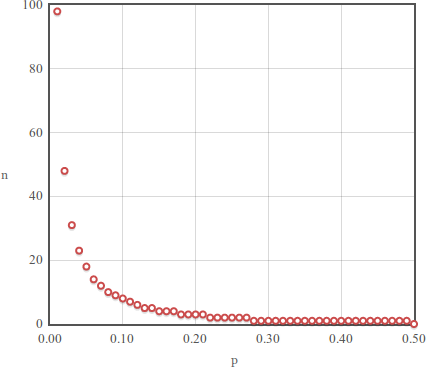
\includegraphics[width=0.76\textwidth]{../images/restriction-least-n.png}}
    \\ \vspace{5mm}
    \subfloat[Range of possible $p$, given a fixed $n$]{\label{fig:sn-restriction-p-range}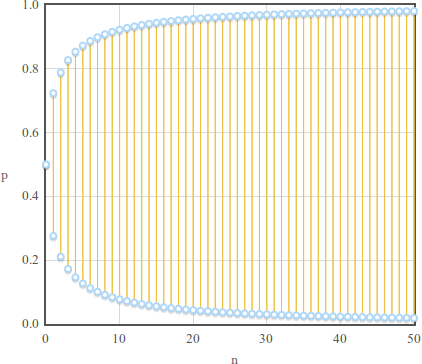
\includegraphics[width=0.76\textwidth]{../images/restriction-p-range.png}}
    \caption{Restrictions on $n$ and $p$ necessary to obtain $\lambda$}
    \label{fig:sn-restriction}
  \end{figure}
}
